\documentclass[slovene,11pt,a4paper]{article}
\usepackage[margin=2cm,bottom=3cm,foot=1.5cm]{geometry}
\setlength{\parindent}{0pt}
\setlength{\parskip}{0.5ex}

\usepackage[pdftex]{graphicx}
\DeclareGraphicsExtensions{.pdf,.png}


\usepackage{amsmath}
\usepackage{amsfonts}
\usepackage{mathrsfs}
\usepackage[usenames]{color}
\usepackage[slovene]{babel}
\usepackage[utf8]{inputenc}
\usepackage{siunitx}

\def\phi{\varphi}
\def\eps{\varepsilon}
\def\theta{\vartheta}

\newcommand{\thisyear}{2024/25}

\renewcommand{\Re}{\mathop{\rm Re}\nolimits}
\renewcommand{\Im}{\mathop{\rm Im}\nolimits}
\newcommand{\Tr}{\mathop{\rm Tr}\nolimits}
\newcommand{\diag}{\mathop{\rm diag}\nolimits}
\newcommand{\dd}{\,\mathrm{d}}
\newcommand{\ddd}{\mathrm{d}}
\newcommand{\ii}{\mathrm{i}}
\newcommand{\lag}{\mathcal{L}\!}
\newcommand{\ham}{\mathcal{H}\!}
\newcommand{\four}[1]{\mathcal{F}\!\left(#1\right)}
\newcommand{\bigO}[1]{\mathcal{O}\!\left(#1\right)}
\newcommand{\sh}{\mathop{\rm sinh}\nolimits}
\newcommand{\ch}{\mathop{\rm cosh}\nolimits}
\renewcommand{\th}{\mathop{\rm tanh}\nolimits}
\newcommand{\erf}{\mathop{\rm erf}\nolimits}
\newcommand{\erfc}{\mathop{\rm erfc}\nolimits}
\newcommand{\sinc}{\mathop{\rm sinc}\nolimits}
\newcommand{\rect}{\mathop{\rm rect}\nolimits}
\newcommand{\ee}[1]{\cdot 10^{#1}}
\newcommand{\inv}[1]{\left(#1\right)^{-1}}
\newcommand{\invf}[1]{\frac{1}{#1}}
\newcommand{\sqr}[1]{\left(#1\right)^2}
\newcommand{\half}{\frac{1}{2}}
\newcommand{\thalf}{\tfrac{1}{2}}
\newcommand{\pd}{\partial}
\newcommand{\Dd}[3][{}]{\frac{\ddd^{#1} #2}{\ddd #3^{#1}}}
\newcommand{\Pd}[3][{}]{\frac{\pd^{#1} #2}{\pd #3^{#1}}}
\newcommand{\avg}[1]{\left\langle#1\right\rangle}
\newcommand{\norm}[1]{\left\Vert #1 \right\Vert}
\newcommand{\braket}[2]{\left\langle #1 \vert#2 \right\rangle}
\newcommand{\obraket}[3]{\left\langle #1 \vert #2 \vert #3 \right \rangle}
\newcommand{\hex}[1]{\texttt{0x#1}}

\renewcommand{\iint}{\mathop{\int\mkern-13mu\int}}
\renewcommand{\iiint}{\mathop{\int\mkern-13mu\int\mkern-13mu\int}}
\newcommand{\oiint}{\mathop{{\int\mkern-15mu\int}\mkern-21mu\raisebox{0.3ex}{$\bigcirc$}}}

\newcommand{\wunderbrace}[2]{\vphantom{#1}\smash{\underbrace{#1}_{#2}}}

\renewcommand{\vec}[1]{\overset{\smash{\hbox{\raise -0.42ex\hbox{$\scriptscriptstyle\rightharpoonup$}}}}{#1}}
\newcommand{\bec}[1]{\mathbf{#1}}


\title{
\sc\large Matematično-fizikalni praktikum \thisyear \\
\bigskip
\bf\Large 8.~naloga: Robni problem lastnih vrednosti
}
\author{}
\date{}


\begin{document}
\maketitle
\vspace{-1cm}

Pri robnem problemu lastnih vrednosti poznamo diferencialno enačbo
in nekaj robnih pogojev (običajno vsaj toliko, kolikor je red enačbe)
Za rešitev problema moramo v splošnem v enem zamahu določiti
tako (lastne) funkcije, ki ustrezajo danim robnim pogojem,
kot (lastne) vrednosti, ki skupaj zadoščajo diferencialni enačbi.
Reševanje robnih problemov je zato lahko bistveno bolj zapleteno
kot integracija začetnih problemov.


Numerično bomo reševali stacionarno Schr\"odingerjevo enačbo
\begin{equation*}
-\frac{\hbar^2}{2m}\,\Dd[2]{\psi}{x} + V(x)\psi = E\psi  
\end{equation*}
za neskončno potencialno jamo ($V(-a/2 < x < a/2)=0$ 
in $V(|x|\ge a/2)\to\infty$) ter za končno potencialno jamo
($V(|x|\ge a/2)=V_0$), za kateri poznamo analitične rešitve;
glej Strnad, {\sl Fizika II\/}.  Dva značilna pristopa, diferenčna
metoda in strelska metoda, nas bosta pripravila na resnejše probleme,
za katere analitičnih rešitev ne poznamo.

Pri {\sl diferenčni metodi\/} razdelimo interval
$[-a/2,a/2]$ na $N$ točk ($x_i = -a/2 + ia/N$) in prepišemo drugi
krajevni odvod v drugo diferenco, tako da ima brezdimenzijska enačba obliko
\begin{equation*}
\frac{\psi_{i-1} - 2\psi_i + \psi_{i+1}}{h^2} + E\psi_i = 0  
\end{equation*}
oziroma
\begin{equation*}
\psi_{i-1} - (2-\lambda)\psi_i + \psi_{i+1} = 0 \>,  
\end{equation*}
kjer je $\lambda=Eh^2=k^2h^2$.  Diskretizirati je treba tudi robna
pogoja pri $x=-a/2$ in $x=a/2$, ki sta v splošnem (in tudi
pri končni jami) mešanega tipa,
\begin{align*}
c_1 \psi_0 + c_2 \frac{\psi_1 - \psi_{-1}}{2h} =& 0 \>, \\
d_1 \psi_N + d_2 \frac{\psi_{N+1} - \psi_{N-1}}{2h} =& 0 \>,
\end{align*}
medtem ko sta pri neskončni jami preprostejša, $\psi_0=\psi_N=0$.
V primerih potencialnih jam tako dobimo tridiagonalni sistem $N$
oziroma $N-1$ linearnih enačb
\begin{equation*}
A \underline{\psi} = \lambda \underline{\psi}   
\end{equation*}
za lastne vektorje $\underline{\psi}$ in lastne vrednosti $\lambda$,
ki ga rešujemo z diagonalizacijo.  

\smallskip

Pri {\sl strelski metodi\/} začnemo s ``kosinusnim'' začetnim pogojem
v izhodišču $\psi(0)=1$, $\psi'(0)=0$ ali ``sinusnim'' pogojem
$\psi(0)=0$, $\psi'(0)=1$, nato pa z nekim izbranim $E$ diferencialno
enačbo s poljubno integracijsko shemo (npr.~RK4) integriramo do roba
$x=a/2$ in tam preverimo, ali je izpolnjen drugi robni pogoj, $\psi(a/2)=0$.
Vrednost $E$ spreminjamo tako dolgo, dokler robni pogoj ni izpolnjen do
zahtevane natančnosti, in tako dobimo sode in lihe rešitve enačbe
skupaj z ustreznimi lastnimi vrednostmi energije.

\medskip

{\it Naloga\/}: Določi nekaj najnižjih lastnih funkcij in lastnih
vrednosti za
neskončno in končno potencialno jamo z diferenčno metodo in metodo streljanja, lahko pa poskusiš še iterativno in  s kakšno drugo metodo. 
Problem končne jame je s strelsko metodo le trivialna posplošitev
problema neskončne jame: spremeni se le robni pogoj pri $x=a/2$,
ki ima zaradi zahteve po zveznosti in zvezni odvedljivosti valovne
funkcije zdaj obliko $c_1\psi(a/2) + c_2\psi'(a/2) = 0$. 
Alternativno, lahko pri končni jami problem obrnemo in začnemo daleč stran, kjer je funkcija 
(in odvod le-te) skoraj nič, ter poskušamo zadeti  pogoj (soda,liha funkcija) v izhodišču. Preveri,
kaj je bolje (bolj stabilno, natančno)!
Kaj ima pri diferenčni metodi večjo vlogo pri napaki:
končna natančnost diference, s katero aproksimiramo drugi odvod,
ali zrnatost intervala (končna razsežnost matrike, ki jo
diagonaliziramo)?

\bigskip

{\it Dodatna naloga\/}: Določi nekaj najnižjih lastnih funkcij $\psi$
in lastnih vrednosti $E=k^4$ diferencialne enačbe
\begin{equation*}
\Dd[4]{\psi}{x} - E\psi = 0
\end{equation*}
(pozor, minus) na intervalu $[-a/2,a/2]$ z robnimi pogoji
\begin{equation*}
\psi(\pm a/2) = \psi''(\pm a/2) = 0
\end{equation*}
z diferenčno metodo oziroma diagonalizacijo.  (Strelska metoda
pri robnih problemih četrtega reda ni najbolj primerna.)
Namesto četrtega odvoda uporabi izraz za četrto diferenco,
tako da ima $i$-ta diferenčna enačba obliko
\begin{equation*}
\psi_{i-2} - 4\psi_{i-1} + 6\psi_i - 4\psi_{i+1} + \psi_{i+2}
= \underbrace{h^4k^4}_\lambda \psi_i \>.  
\end{equation*}
Ko diskretiziraš še robne pogoje, podobno kot pri enačbi
drugega reda rešuješ petdiagonalni sistem linearnih enačb.
\section{Rešitev}

Najprej si poglejmo avtokorelacijo za obe sovi.
\begin{figure}[h]
    \centering
    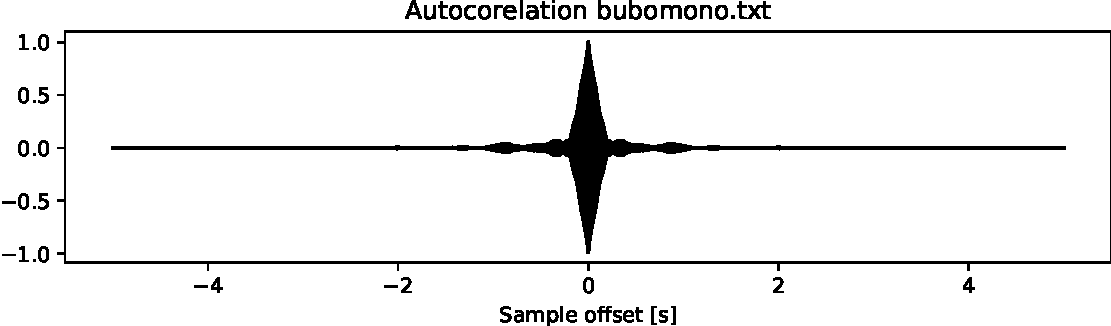
\includegraphics[width=12cm]{pdfs/bubomono.txt_acor.pdf}
    \vspace{10pt}
    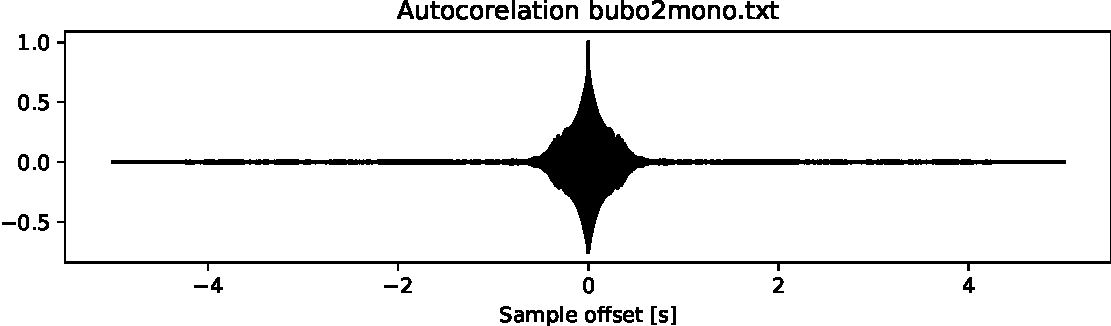
\includegraphics[width=12cm]{pdfs/bubo2mono.txt_acor.pdf}
    \caption{Avtokorelacija signala sov}
\end{figure}

Preden sem koreliral signal sem vektorja samplov normiral, tako da je
"najmočnejši" signal 1. To pomeni \[\|x\|_\infty = \max_i |x_i|\]

Poglejmo si še korelacije med sovami in posnetki:
\newpage
\begin{figure}[h]
    \centering
    \foreach \mix in {mix, mix1, mix2, mix22} {
        \foreach \sova in {bubomono, bubo2mono}{
            \includegraphics[width=8cm]{pdfs/cor_\mix.txt_\sova.txt.pdf}
        }
    }
    \caption{Korelacija sov in posnetkov iz narave}
\end{figure}
Tukaj je bila normalizacija drugače izbrana. Tukaj je bila narejena normalizacija korelacije. Če je varianca signala a $\sigma_a$,
potem je $ \mathbf{x} = \mathbf{x} / \left(\sigma_a \sigma_b |\mathbf{b}|\right)$. Sigma je izračunana z \verb|numpy.std()|.


Hitrosti so precej dolgčasno pričakovane ampak vseeno.
\begin{figure}[h]
    \centering
    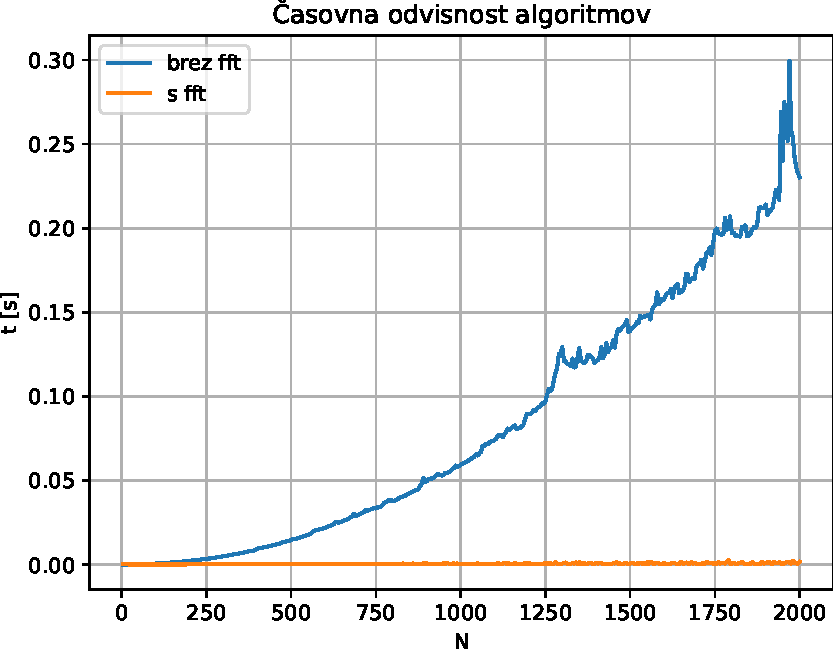
\includegraphics[width=8cm]{pdfs/cas-lin.pdf}
    \vspace{10pt}
    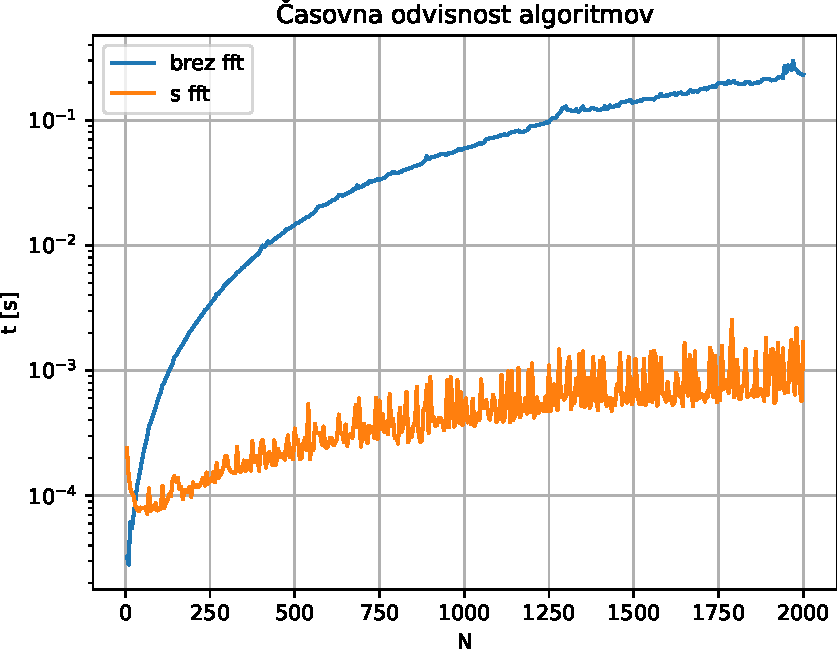
\includegraphics[width=8cm]{pdfs/cas-log.pdf}
    \caption{Hitrost algoritmov}
\end{figure}
\newpage
\section{Dodatna naloga}
Posnel sem dva človeka m in ž ko izgovarjata aaaaaaaaaaaa. Posnel sem jih tudi
ko bereta slovar. Gledal sem ali lahko spet zaznam ali gre za ž glas ali m glas.
Poglejmo si spektra njunega glasu.
\begin{figure}[h]
    \begin{center}
        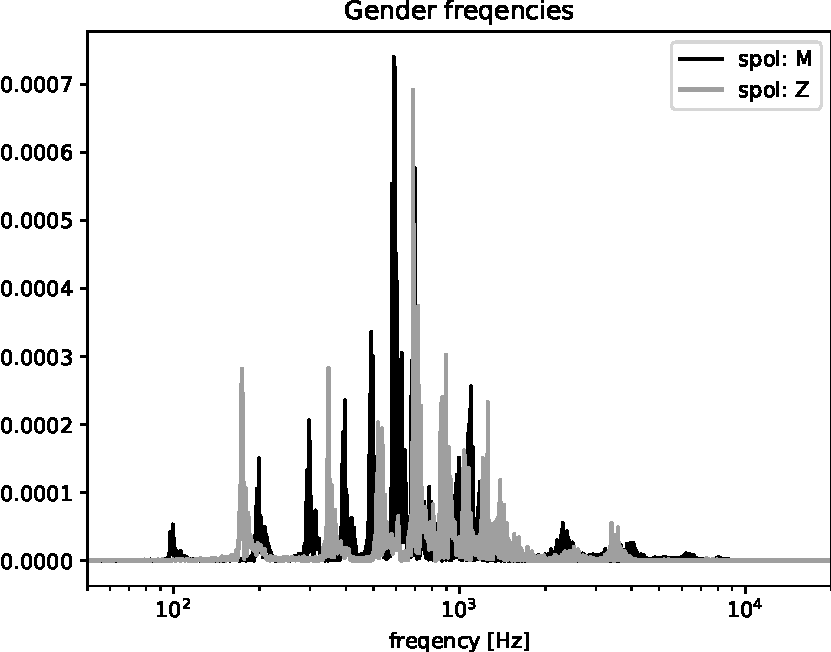
\includegraphics[width=12cm]{pdfs/fft_spol.pdf}
    \end{center}
    \caption{Barva glasu moškega in ženske}
\end{figure}

% Glasova sta bila prej normirana, saj je bil moški glas posnet bližje mikrofona.
% Poglejmo si zopet korelacijo med posnetki:
% \foreach \gender in {Z, M} {
%     \foreach \mix in {Glas\ 001, Glas\ 002}{
%         pdfs/cor_\gender_\mix.pdf 
%     }
% }
\begin{figure}[h]
    \begin{center}
        
    \foreach \gender in {Z, M} {%
        \foreach \mix in {001, 002} {%
            \includegraphics[width=8cm]{pdfs/cor_\gender_Glas\space\mix.pdf}%    
        }%
        \par
}%
    \end{center}
    
    \caption{Korelacija glasa človeka in posnetkov iz branja slovarja}
\end{figure}
\end{document}
